\documentclass[11pt,a4paper]{article}
\usepackage[T1]{fontenc}
\usepackage[utf8]{inputenc}
\usepackage{lmodern}
\usepackage[margin=2.4cm]{geometry}
\usepackage{amsmath,amssymb}
\usepackage{booktabs}
\usepackage{graphicx}
\usepackage{caption}
\usepackage{microtype}
\usepackage{enumitem}
\usepackage{xcolor}
\usepackage[colorlinks=true,linkcolor=blue!50!black,urlcolor=blue!50!black]{hyperref}
\setlist{itemsep=2pt,topsep=4pt}
\captionsetup{font=small,labelfont=bf}

\title{\textbf{Predicting Recall in Spaced Repetition:\\A Bayesian Model, FSRS-6 and Gradient-Boosted Trees}\\[4pt]
\large Axiom FYP --- Summary}
\author{}
\date{November 2026}

\begin{document}
\maketitle

\begin{abstract}
\noindent We compare four ways of predicting whether a learner will recall a flashcard at a review: Half-Life Regression (HLR), FSRS-6
(with default and with per-user optimised weights), our continuous-time hierarchical Bayesian state-space model fitted by MCMC (v1), and a
gradient-boosted tree model (GBDT) with no memory equation. All are scored one step ahead on the same held-out reviews of two datasets, 100
Anki users and the full Duolingo traces. The GBDT has the best value of every metric on both datasets, up to a tie in the Anki mean bias (log loss 0.358 on Anki and 0.259 on
Duolingo). Among the other models, FSRS-6 (optimised) is best on Anki and the Bayesian model v1 is best on Duolingo, so that ranking depends on
the dataset. The Bayesian model's chains did not converge, so its scores are provisional. We report the leakage and selection issues that
affect the result.
\end{abstract}

\section{Problem}
A spaced-repetition scheduler needs, for each review, the probability that the learner recalls the item given the card's earlier reviews and
the time since the last one. We treat this as binary prediction: at each scored review the model outputs a recall probability using only
reviews that precede it, and the probability is scored against the recorded outcome. A better probability should make better schedules possible,
but no scheduling simulation was run here.\footnote{This summary covers HLR, FSRS-6, v1 and the GBDT only. Further model variants are in the full black-book report.}

\section{Data}
\textbf{Anki.} 100 users sampled with seed 0 from the public \texttt{anki-revlogs-10k} collection, with at most 1000 cards per user: 99,074 cards and
768,658 review events. The outcome is binary: a review is recalled if its grade is above Again.\\
\textbf{Duolingo.} The full half-life regression traces of Settles and Meeder: 115,222 users, 5,861,629 cards (a card is a user--lexeme pair) and
12,854,226 events. The outcome is binary by construction, so FSRS-6 sees only Again and Good here.

\section{Protocol}
For each user the cutoff is the 80th percentile of that user's day offsets. Reviews before it are training data and later reviews are test data
(Anki: 606,364 training and 162,294 test events; Duolingo: 6,468,512 and 6,385,714). A test review is scored only if it is not the card's first review and its elapsed time is at
least one day. This leaves 95,400 scored reviews on Anki (recall rate 0.831) and 1,189,355 on Duolingo (recall rate 0.920). Every model is fitted on the training events only,
and predicts each scored review from the history before it. Parameters are frozen after fitting.

We report six metrics: log loss, the Brier score, AUC, expected calibration error (ECE), the root mean squared error over calibration bins (RMSE$_{\mathrm{bins}}$), and the mean bias
(mean predicted recall minus observed recall). Differences between models are tested by a paired, user-clustered bootstrap (1000 resamples, seed 0), and a difference is called
significant only if its 95\% interval excludes zero (marked by an asterisk).

\section{The four models}
\textbf{HLR} (Half-Life Regression) predicts recall as $2^{-\Delta t/h}$ with a half-life $h$ that is a function of the numbers of correct and incorrect earlier answers, fitted by
stochastic gradient descent. It is the oldest and simplest trainable baseline.

\textbf{FSRS-6} keeps a per-card memory state of stability and difficulty, updates it after each review with a fixed functional form, and reads recall from a power forgetting curve. We use the
py-fsrs implementation with its 21 default weights (default) and with the weights fitted per user on that user's training reviews (optimised). A user with too few informative training reviews
keeps the defaults.

\textbf{v1, the Bayesian model.} Each card sequence has one latent logit state that follows a mean-reverting Ornstein--Uhlenbeck process between reviews, with an exact closed-form transition over any
gap. Recall is a Bernoulli outcome through the logistic link. The equilibrium mean is a hierarchy of global, user and item effects with a user slope on the lagged outcome, and the decay rate may depend on
practice. Inference is a Metropolis-within-Gibbs sampler with P\'olya--Gamma augmentation, forward filtering and backward sampling of the latent paths, conjugate updates and random-walk Metropolis steps (2000
iterations, 1000 burn-in, one chain, seed 0). On Duolingo the GPU port of the same sampler was used. Predictions average over the posterior draws (250 on Anki, 100 on Duolingo). It uses the binary outcome only.

\textbf{GBDT} is a LightGBM model with no memory equation. For each review it uses past-only features: the gap since the card's previous review, the card's history (counts, lapses, last three grades, outcomes and gaps), the
FSRS-6 default state (stability, difficulty, retrievability) replayed over the card's history, running statistics of the user's recall so far, and, on Duolingo, a smoothed recall rate of the item. It is trained on all
non-first reviews (15 leaves per tree, learning rate 0.02, early stopping on a holdout of the fit data). The configuration was chosen on validation data only (the last 20\% of each user's training days).

\section{Results}
Tables~\ref{tab:anki} and~\ref{tab:duo} give the overall metrics, and Figure~\ref{fig:ll} shows the log losses. Arrows show the direction of improvement; for the mean bias the best value is the one closest to zero. On Anki the GBDT ($+0.0016$ unrounded) and FSRS-6 (optimised) ($-0.0019$) tie at three decimals, and the GBDT is bolded because it is closer to zero.

\begin{table}[htbp]
  \centering
  \caption{Anki: overall metrics on 95,400 scored reviews. Bold marks the best value in each column.}
  \label{tab:anki}
  \small
  \begin{tabular}{@{}lcccccc@{}}
    \toprule
    Model & Log loss $\downarrow$ & Brier $\downarrow$ & AUC $\uparrow$ & ECE $\downarrow$ & RMSE$_{\mathrm{bins}}$ $\downarrow$ & $|$Mean bias$|$ $\to 0$ \\
    \midrule
    HLR & 0.680 & 0.170 & 0.555 & 0.146 & 0.176 & $+0.060$ \\
    FSRS-6 (default) & 0.396 & 0.121 & 0.745 & 0.012 & 0.017 & $+0.011$ \\
    FSRS-6 (optimised) & 0.379 & 0.117 & 0.777 & 0.009 & 0.014 & $-0.002$ \\
    v1 (Bayesian MCMC) & 0.422 & 0.131 & 0.692 & 0.025 & 0.032 & $+0.011$ \\
    GBDT & \textbf{0.358} & \textbf{0.111} & \textbf{0.805} & \textbf{0.005} & \textbf{0.010} & \textbf{$+0.002$} \\
    \bottomrule
  \end{tabular}
\end{table}

\begin{table}[htbp]
  \centering
  \caption{Duolingo: overall metrics on 1,189,355 scored reviews. Bold marks the best value in each column. The v1 row is the GPU port.}
  \label{tab:duo}
  \small
  \begin{tabular}{@{}lcccccc@{}}
    \toprule
    Model & Log loss $\downarrow$ & Brier $\downarrow$ & AUC $\uparrow$ & ECE $\downarrow$ & RMSE$_{\mathrm{bins}}$ $\downarrow$ & $|$Mean bias$|$ $\to 0$ \\
    \midrule
    HLR & 0.418 & 0.079 & 0.521 & 0.072 & 0.072 & $+0.072$ \\
    FSRS-6 (default) & 0.302 & 0.078 & 0.566 & 0.051 & 0.070 & $-0.025$ \\
    FSRS-6 (optimised) & 0.300 & 0.078 & 0.570 & 0.050 & 0.070 & $-0.026$ \\
    v1 (Bayesian MCMC) & 0.268 & 0.071 & 0.656 & 0.014 & 0.017 & $+0.004$ \\
    GBDT & \textbf{0.259} & \textbf{0.070} & \textbf{0.697} & \textbf{0.001} & \textbf{0.003} & \textbf{$+0.000$} \\
    \bottomrule
  \end{tabular}
\end{table}

\begin{figure}[htbp]
  \centering
  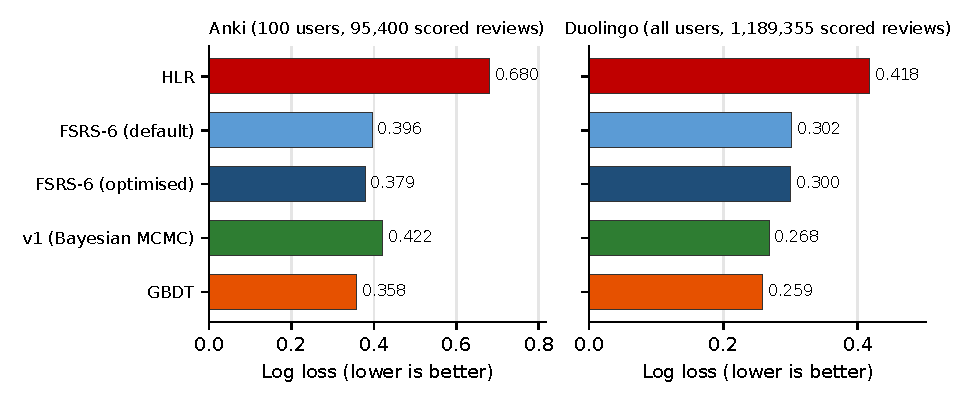
\includegraphics[width=0.95\textwidth]{summary_log_loss.pdf}
  \caption{Overall log loss of the five models on Anki (left) and on Duolingo (right). Each bar starts at zero.}
  \label{fig:ll}
\end{figure}

On Anki, the GBDT is best on every column of Table~\ref{tab:anki}, with log loss 0.358 against 0.379 for FSRS-6 (optimised) and 0.422 for v1. FSRS-6 (optimised) is the best of the other four, and v1 sits between FSRS-6 and HLR. On Duolingo, the GBDT is again best on every metric (log loss 0.259),
followed by v1 (0.268), while FSRS-6 (optimised) has 0.300. The order of FSRS-6 and v1 therefore reverses between the two datasets.

\subsection{Paired differences and user wins}
Table~\ref{tab:paired} gives the paired log-loss difference of each model against FSRS-6 (optimised); negative favours the model.

\begin{table}[htbp]
  \centering
  \caption{Paired log-loss difference, model minus FSRS-6 (optimised), with 95\% user-clustered bootstrap intervals. An asterisk marks an interval that excludes zero. The last row is the GBDT minus v1 on Anki.}
  \label{tab:paired}
  \small
  \begin{tabular}{@{}lcc@{}}
    \toprule
    Model & Anki & Duolingo \\
    \midrule
    HLR & $+0.301$ [$+0.246$, $+0.361$]$^{*}$ & $+0.118$ [$+0.112$, $+0.124$]$^{*}$ \\
    FSRS-6 (default) & $+0.017$ [$+0.008$, $+0.025$]$^{*}$ & $+0.002$ [$+0.001$, $+0.002$]$^{*}$ \\
    v1 (Bayesian MCMC) & $+0.043$ [$+0.033$, $+0.055$]$^{*}$ & $-0.032$ [$-0.033$, $-0.031$]$^{*}$ \\
    GBDT & $-0.021$ [$-0.028$, $-0.014$]$^{*}$ & $-0.041$ [$-0.042$, $-0.041$]$^{*}$ \\
    \midrule
    GBDT minus v1 & $-0.064$ [$-0.078$, $-0.052$]$^{*}$ & -- \\
    \bottomrule
  \end{tabular}
\end{table}

Per user, the GBDT has lower log loss than FSRS-6 (optimised) for 82 of the 100 Anki users and for 78.0\% of the 41,223 Duolingo users, and it beats v1 on 94 of the 100 Anki users.

\section{Overfitting checks}
All checks use data the model did not see. The GBDT's validation log loss on Anki is 0.3614 and its test log loss is 0.3584. On Duolingo the validation value (a 5,000-user development sample) is 0.2578 and the test value (all users) is 0.2588.
On Anki its log loss on its own training rows (341,739 rows) is 0.3467, against 0.3584 on the test rows. Among the scored Duolingo users, 2,004 have no training rows (15,918 scored reviews; 64,254 users overall have none), and on them the GBDT has log loss 0.2329, against 0.2647 for v1 and 0.2748 for
FSRS-6 (optimised) on Duolingo, so its lead is largest on users it has never seen. The GBDT's gain comes mostly from running statistics of the user's own performance (dropping that feature group raises the Anki validation log loss from 0.363 to 0.377) and from training on all non-first reviews,
and not from a memory model.

\section{Key disclosures}
\begin{itemize}
  \item \textbf{A same-session leak was found and fixed.} Duolingo logs one practice session at a single timestamp, and a first version of the GBDT used outcomes from the same session. Its development log loss of 0.2473 was invalid. After grouping rows with the same timestamp it is 0.2578. All GBDT numbers here use the fixed version.
  \item \textbf{The test set was looked at twice.} The GBDT configuration was frozen before its test run, but an earlier model was scored on the same test data in an earlier phase, and many variants were tried during selection, so the validation numbers are optimistic.
  \item \textbf{v1 did not converge.} On Duolingo the learned rate $\lambda$ of v1 did not converge, and no run met the convergence gate, so the v1 scores are provisional.
  \item \textbf{FSRS-6 (optimised) is nearly the default model on Duolingo.} It kept the default weights for 115,110 of 115,222 users, so its Duolingo numbers are mostly those of the defaults.
  \item \textbf{Lexeme pooling.} The Duolingo item recall rate pools training rows of other users that fall later in calendar time, an effect of about 0.001 in log loss that we accepted.
  \item \textbf{Scope.} One seed and one split, 100 Anki users, and no scheduling simulation. The GBDT is a pure predictor with no memory state, so it cannot by itself drive a scheduler, whereas v1 keeps an interpretable latent state.
\end{itemize}

\section{Conclusion}
In these experiments a tree model with no memory equation is the most accurate predictor on both datasets (up to the tie in the Anki mean bias), ahead of FSRS-6 and of the Bayesian model, and its paired differences against FSRS-6 (optimised) exclude zero on both. Its advantage comes from information about the
learner's own recent performance, which the card-level memory models do not use, and not from better memory modelling. The Bayesian model beats HLR on both datasets, loses to FSRS-6 (optimised) on Anki and beats it on Duolingo, where the comparison is weakened by
FSRS-6 falling back to default weights and by the unconverged chains. Which kind of model gives better schedules remains untested. The sampler fit takes about 7.6 hours on one CPU core for the Anki run (2,598 seconds on the GPU for Duolingo), against under a minute for the GBDT on Anki (26.8 seconds) and 265 seconds on Duolingo.

\end{document}
